\documentclass[12pt]{article}
\usepackage[ukrainian,shorthands=off]{babel}   % shorthands=off: символ " не активний (потрібно для міток "..." у TikZ всередині \zadtask)
\usepackage{fontspec}
% --- НАЛАШТУВАННЯ ШРИФТІВ ---
% Шрифти Schoolbook-*.otf лежать у корені проєкту. Шлях підбирається автоматично:
% ../ (компіляція з папки теми), ./ (корінь проєкту), ../../ (підпапки теми 28); інакше -- TeX Gyre Schola.
\newcommand{\nmtSchoolbook}[1]{\setmainfont{Schoolbook-Regular.otf}[
    Path = #1,
    BoldFont = Schoolbook-Bold.otf,
    ItalicFont = Schoolbook-Italic.otf,
    BoldItalicFont = Schoolbook-BoldItalic.otf
]}
\IfFileExists{../Schoolbook-Regular.otf}{\nmtSchoolbook{../}}{%
 \IfFileExists{./Schoolbook-Regular.otf}{\nmtSchoolbook{./}}{%
  \IfFileExists{../../Schoolbook-Regular.otf}{\nmtSchoolbook{../../}}{%
   \setmainfont{texgyreschola}[Extension=.otf, UprightFont=*-regular, BoldFont=*-bold, ItalicFont=*-italic, BoldItalicFont=*-bolditalic]}}}
\usepackage[italic]{mathastext}
\usepackage[a4paper,margin=1.8cm,bottom=2cm,top=2cm]{geometry}
\usepackage{amsmath,amssymb}
\usepackage{tikz}
\usepackage{pgfplots}
\pgfplotsset{compat=1.18}
\usepgfplotslibrary{fillbetween}
\usetikzlibrary{calc,patterns,angles,quotes,intersections,babel,3d,shapes.symbols,shapes.geometric,decorations.pathreplacing,shadings,arrows.meta,hobby}
\usepackage{xcolor,array,fancyhdr,enumitem,multicol}
\usepackage{colortbl,multirow,diagbox,needspace}
\usepackage{tcolorbox}
\tcbuselibrary{skins,breakable}
\usepackage[hidelinks]{hyperref}
% водяний знак; щоб зібрати без нього (версія для вчителів), перед \documentclass пишуть \def\nmtnowatermark{}
\ifdefined\nmtnowatermark\else
\usepackage[firstpage=false, text=@pvtr2525, scale=0.6, color=gray!12]{draftwatermark}
\fi

% --- АВТОСТИСКАННЯ: рисунок/сітка, ширша за колонку, масштабується до ширини колонки ---
\newsavebox{\nmtfitbox}
\newenvironment{nmtfit}{\begin{lrbox}{\nmtfitbox}}{\end{lrbox}%
  \ifdim\wd\nmtfitbox>\linewidth \resizebox{\linewidth}{!}{\usebox{\nmtfitbox}}\else\usebox{\nmtfitbox}\fi}
\let\nmtIncludegraphicsOrig\includegraphics
\renewcommand{\includegraphics}[2][]{\begin{nmtfit}\nmtIncludegraphicsOrig[#1]{#2}\end{nmtfit}}


\definecolor{mainGreen}{RGB}{34, 120, 64}
\definecolor{yearOrange}{RGB}{220, 100, 30}
\definecolor{yearcolor}{RGB}{220, 100, 30}
\definecolor{titleBg}{RGB}{225, 240, 220}
\definecolor{instrBg}{RGB}{255, 240, 220}
\definecolor{instrBorder}{RGB}{220, 150, 80}
\definecolor{headerblue}{RGB}{0, 102, 204}   % використовується в рисунках старої бази

\setlength{\parindent}{0pt}
\emergencystretch=1.5em

\pagestyle{fancy}
\fancyhf{}
\renewcommand{\headrulewidth}{0.4pt}
\renewcommand{\footrulewidth}{0.4pt}
\fancyhead[C]{\small\color{gray!80} Геометрія: завдання на відповідність з обчисленням площ}
\fancyhead[R]{\small\color{mainGreen}\textbf{\href{https://t.me/pvtr2525}{@pvtr2525}}}
\fancyfoot[L]{\small\color{gray!80}\href{https://t.me/pvtr2525}{ТГ: @pvtr2525}}
\fancyfoot[C]{\small\color{gray!80}\thepage}
\fancyfoot[R]{\small\color{gray!80}НМТ 2022--2026}

% --- ТАБЛИЦІ ВІДПОВІДЕЙ ---
% ширина клітинки = (ширина рядка - відступи) / 5: на всю сторінку це ~3 см, у minipage поруч із рисунком таблиця стискається;
% п'ять колонок |m{w}| мають 10 відступів \tabcolsep і 6 вертикальних ліній -- тоді таблиця рівно на \linewidth
\newlength{\nmtcellw}
\newcommand{\nmtSetCell}{\setlength{\nmtcellw}{\dimexpr(\linewidth-10\tabcolsep-6\arrayrulewidth)/5\relax}}
\newcommand{\answerTable}[5]{%
\par\nopagebreak\vspace{0.15cm}
\noindent\nmtSetCell
\begin{tabular}{|*{5}{>{\centering\arraybackslash}m{\nmtcellw}|}}
\hline
\rule[-0.15cm]{0pt}{0.6cm}\textbf{А} & \rule[-0.15cm]{0pt}{0.6cm}\textbf{Б} & \rule[-0.15cm]{0pt}{0.6cm}\textbf{В} & \rule[-0.15cm]{0pt}{0.6cm}\textbf{Г} & \rule[-0.15cm]{0pt}{0.6cm}\textbf{Д} \\
\hline
\rule[-0.2cm]{0pt}{0.75cm}#1 & \rule[-0.2cm]{0pt}{0.75cm}#2 & \rule[-0.2cm]{0pt}{0.75cm}#3 & \rule[-0.2cm]{0pt}{0.75cm}#4 & \rule[-0.2cm]{0pt}{0.75cm}#5 \\
\hline
\end{tabular}
\par\vspace{0.25cm}
}
\newcommand{\answerTableTall}[5]{%
\par\nopagebreak\vspace{0.15cm}
\noindent\nmtSetCell
\begin{tabular}{|*{5}{>{\centering\arraybackslash}m{\nmtcellw}|}}
\hline
\rule[-0.2cm]{0pt}{0.7cm}\textbf{А} & \rule[-0.2cm]{0pt}{0.7cm}\textbf{Б} & \rule[-0.2cm]{0pt}{0.7cm}\textbf{В} & \rule[-0.2cm]{0pt}{0.7cm}\textbf{Г} & \rule[-0.2cm]{0pt}{0.7cm}\textbf{Д} \\
\hline
\rule[-0.45cm]{0pt}{1.2cm}#1 & \rule[-0.45cm]{0pt}{1.2cm}#2 & \rule[-0.45cm]{0pt}{1.2cm}#3 & \rule[-0.45cm]{0pt}{1.2cm}#4 & \rule[-0.45cm]{0pt}{1.2cm}#5 \\
\hline
\end{tabular}
\par\vspace{0.25cm}
}
\newcommand{\instructionBox}[1]{%
\par\vspace{0.3cm}
\begin{tcolorbox}[colback=instrBg, colframe=instrBorder, boxrule=0.6pt, arc=2pt,
    left=8pt, right=8pt, top=4pt, bottom=4pt]
\centering\small\bfseries #1
\end{tcolorbox}
\par\vspace{0.15cm}
}
\newcommand{\sectionTitle}[1]{%
\par\vspace{0.4cm}
\begin{tcolorbox}[colback=titleBg, colframe=titleBg, boxrule=0pt, arc=8pt,
    halign=center, fontupper=\Large\bfseries\color{mainGreen}]
\hyphenpenalty=10000 \exhyphenpenalty=10000 #1
\end{tcolorbox}
\par\vspace{0.3cm}
}
\newcommand{\task}[2]{\noindent\textbf{#1.}\ \ #2\par\vspace{0.2cm}}
% --- НМТ-СТИЛЬ ПОЛЕ ВІДПОВІДІ ---
\newcommand{\nmtAnswerBox}{%
\par\nopagebreak\vspace{0.2cm}\noindent
Відповідь:\ \
\begin{tabular}{@{}*{4}{|>{\centering\arraybackslash}p{0.8cm}}|@{\hspace{0.1cm}\textbf{,}\hspace{0.1cm}}*{3}{|>{\centering\arraybackslash}p{0.8cm}}|@{}}
\hline
\rule[-0.2cm]{0pt}{0.7cm} & & & & & & \\
\hline
\end{tabular}
\par\vspace{0.3cm}
}
% --- СІТКА ДЛЯ МАТЧИНГУ ---
\newsavebox{\nmtgridbox}
\newcommand{\matchingGrid}{%
    \sbox{\nmtgridbox}{\matchingGridRaw}%
    \ifdim\wd\nmtgridbox>\linewidth \resizebox{\linewidth}{!}{\usebox{\nmtgridbox}}\else\usebox{\nmtgridbox}\fi}
\newcommand{\matchingGridRaw}{%
    \begingroup
    \renewcommand{\arraystretch}{1.15}
    \setlength{\tabcolsep}{4pt}
    \footnotesize
    \begin{tabular}{r|c|c|c|c|c|}
         \multicolumn{1}{c}{} & \multicolumn{1}{c}{\textbf{А}} & \multicolumn{1}{c}{\textbf{Б}} & \multicolumn{1}{c}{\textbf{В}} & \multicolumn{1}{c}{\textbf{Г}} & \multicolumn{1}{c}{\textbf{Д}} \\ \cline{2-6}
         \textbf{1} & \phantom{X} & \phantom{X} & \phantom{X} & \phantom{X} & \phantom{X} \\ \cline{2-6}
         \textbf{2} & & & & & \\ \cline{2-6}
         \textbf{3} & & & & & \\ \cline{2-6}
    \end{tabular}
    \endgroup
}
% --- ДОДАТКОВІ МАКРОСИ ЗБІРНИКА ---
\newcommand{\taskBlock}[1]{%
\par\vspace{0.45cm}
\noindent{\color{mainGreen}\rule{\linewidth}{0.8pt}}\par\vspace{0.12cm}
\noindent{\small\bfseries\color{mainGreen}#1}\par\vspace{0.25cm}
}
\newcounter{zad}
\newcommand{\zadtask}[1]{\stepcounter{zad}\noindent\textbf{\thezad.}\ \ #1\par\nopagebreak\vspace{0.2cm}}
\newcommand{\zadnum}{\stepcounter{zad}\textbf{\thezad.}\ \ }
\newcounter{ans}
\newcommand{\ansitem}[1]{\stepcounter{ans}\noindent\textbf{\theans.}\ #1\par\vspace{0.07cm}}
% мітка року: нерозривна, притиснута праворуч; якщо не вміщається -- праворуч на новому рядку
\newcommand{\nmtyear}[1]{\unskip\nobreak\finalhyphendemerits=0 \hfill\penalty100\hskip1em\hbox{}\nobreak\hfill{\small\color{yearOrange}\mbox{\rule{0pt}{2.3ex}(НМТ~#1)}}}
% --- МАКРОС КОРОТКОГО РОЗВ'ЯЗКУ ---
\newcommand{\solution}[1]{%
\par\vspace{0.12cm}
\begin{tcolorbox}[colback=titleBg!45, colframe=mainGreen!55, boxrule=0.4pt, arc=2pt,
    left=6pt, right=6pt, top=3pt, bottom=3pt, breakable]
\footnotesize\textbf{Короткий розв'язок.}\ #1
\end{tcolorbox}
\par\vspace{0.12cm}
}
% Розв'язки й відповіді (є до завдань НМТ-2026): \showsolutionstrue -- показати, \showsolutionsfalse -- сховати
\newif\ifshowsolutions
\showsolutionsfalse
% --- ЗАГОЛОВКИ З ПУНКТАМИ КЛІКАБЕЛЬНОГО ЗМІСТУ ---
\setcounter{tocdepth}{2}
\newcommand{\chapterTitle}[1]{%
\clearpage\phantomsection\addcontentsline{toc}{section}{#1}%
\sectionTitle{#1}}
\newcommand{\typeTitle}[1]{%
\needspace{6\baselineskip}%
\phantomsection\addcontentsline{toc}{subsection}{\quad #1}%
\par\vspace{0.3cm}
\noindent{\large\bfseries\color{yearOrange}#1}\par\vspace{0.08cm}
\noindent{\color{yearOrange}\rule{\linewidth}{0.4pt}}\par\nopagebreak\vspace{0.2cm}}
\raggedbottom
% усередині одного завдання сторінка не розривається: нерозривний вертикальний проміжок
% і нерозривна межа абзаців (умова ніколи не відділяється від варіантів, рисунка чи сітки)
\newcommand{\nbvspace}[1]{\nopagebreak\vspace{#1}}
\newcommand{\nmtnobreak}{\ifvmode\penalty10000 \fi}
% --- ЄДИНИЙ МАКЕТ ЗАВДАНЬ НА ВІДПОВІДНІСТЬ ---
% мітка в колонці сталої ширини, текст -- у parbox: продовження довгого рядка
% вирівнюється під текстом, а не під міткою; відступ між пунктами однаковий скрізь
\newlength{\nmtMatchLab}\setlength{\nmtMatchLab}{1.6em}
\newlength{\nmtMatchSep}\setlength{\nmtMatchSep}{0.28cm}
\newcommand{\matchHead}[1]{\par\noindent\textit{#1}\par\nopagebreak\vspace{0.2cm}}
% шаблонний заголовок стовпця зі старого макета -- лише коли завдання не має власного \matchHead
\makeatletter\newcommand{\nmtHeadUnless}[2]{\in@{\matchHead}{#1}\ifin@\else#2\fi}\makeatother
\newcommand{\matchItem}[2]{\par\noindent\makebox[\nmtMatchLab][l]{\textbf{#1}}%
\parbox[t]{\dimexpr\linewidth-\nmtMatchLab\relax}{\raggedright #2}\par\nopagebreak\vspace{\nmtMatchSep}}
\newcommand{\ansTheme}[1]{\par\vspace{0.25cm}\noindent{\bfseries\color{mainGreen}#1}\par\vspace{0.12cm}}
\newcommand{\ansType}[1]{\par\vspace{0.1cm}\noindent{\itshape\color{yearOrange}#1}\par\vspace{0.08cm}}

% варіанти відповіді окремими рядками (довгі вирази не влазять у клітинки таблиці)
\newcommand{\answerRows}[5]{\par\nopagebreak\vspace{0.15cm}%
\matchItem{А}{#1}\matchItem{Б}{#2}\matchItem{В}{#3}\matchItem{Г}{#4}\matchItem{Д}{#5}}
\graphicspath{{./}{10. Основи планіметрії/}{11. Трикутники/}{12. Паралелограм/}{13. Прямокутник/}{16. Трапеція/}}

\begin{document}
\begingroup\setcounter{zad}{0}
% --- макроси з файлів сесій НМТ-2026 (для рисунків) ---
\renewcommand{\headrulewidth}{0.4pt}
\renewcommand{\footrulewidth}{0.4pt}
\definecolor{gold}{RGB}{240, 190, 40}
\definecolor{silver}{RGB}{170, 170, 175}
\definecolor{bronze}{RGB}{190, 120, 70}
\definecolor{hexcol}{RGB}{200,110,60}
\newcommand{\hexthree}[2]{%
    \draw[hexcol, line width=1.1pt]
        ($(#1,#2)+(0:30)$) -- ($(#1,#2)+(60:30)$) -- ($(#1,#2)+(120:30)$) --
        ($(#1,#2)+(180:30)$) -- ($(#1,#2)+(240:30)$) -- ($(#1,#2)+(300:30)$) -- cycle;
}

% --- сумісність зі старою базою (діє, якщо тема не має власного визначення) ---
\providecommand{\trigStyle}[1]{#1}
\providecommand{\answerTableSmall}[5]{%
\begingroup\setlength{\tabcolsep}{2pt}\small\nmtSetCell
\begin{tabular}{|*{5}{>{\centering\arraybackslash}m{\nmtcellw}|}}
\hline
\rule[-0.2cm]{0pt}{0.6cm}\textbf{А} & \textbf{Б} & \textbf{В} & \textbf{Г} & \textbf{Д} \\
\hline
\rule[-0.4cm]{0pt}{0.9cm}#1 & \rule[-0.4cm]{0pt}{0.9cm}#2 & \rule[-0.4cm]{0pt}{0.9cm}#3 & \rule[-0.4cm]{0pt}{0.9cm}#4 & \rule[-0.4cm]{0pt}{0.9cm}#5 \\
\hline
\end{tabular}\endgroup}
\providecommand{\matchingLayout}[3]{%
    \noindent
    \begin{minipage}[t]{0.36\textwidth}\vspace{0pt}\raggedright
        #1
    \end{minipage}%
    \hfill
    \begin{minipage}[t]{0.43\textwidth}\vspace{0pt}\raggedright
        #2
    \end{minipage}%
    \hfill
    \begin{minipage}[t]{0.19\textwidth}
        \vspace{0pt}
        \begin{flushright}
        #3
        \end{flushright}
    \end{minipage}}
\providecommand{\matchingLayoutBottom}[2]{%
    \noindent
    \begin{minipage}[t]{0.48\textwidth}\vspace{0pt}\raggedright
        #1
    \end{minipage}%
    \hfill
    \begin{minipage}[t]{0.48\textwidth}\vspace{0pt}\raggedright
        #2
    \end{minipage}
    \vspace{0.5cm}
    \noindent
    \matchingGrid}
\providecommand{\answerListVertical}[5]{%
    \par\nopagebreak\vspace{0.2cm}
    \begin{itemize}[itemsep=0.4cm, leftmargin=1.5cm, labelsep=0.5cm]
        \item[\textbf{А}] #1
        \item[\textbf{Б}] #2
        \item[\textbf{В}] #3
        \item[\textbf{Г}] #4
        \item[\textbf{Д}] #5
    \end{itemize}
    \vspace{0.2cm}}

\graphicspath{{./}{11. Трикутники/}}
\setcounter{zad}{0}

\chapterTitle{Геометрія: завдання на відповідність з обчисленням площ}

\noindent{\small Збірник містить \textbf{7 справжніх завдань} НМТ 2024--2026 років на встановлення відповідності з планіметрії, у яких \textit{треба знайти площу}: трикутників, частин прямокутника, паралелограма, трапеції, фігур між паралельними прямими й на папері в клітинку. Таких завдань у НМТ 2023--2026 небагато, тому наприкінці додано \textbf{4 авторські аналоги} за зразком НМТ. Завдання згруповано за фігурою; біля кожного оригіналу вказано рік. Відповіді~--- на останній сторінці. Завдання на відповідність без площ~--- в окремому збірнику «Геометрія: завдання на відповідність без обчислення площ».\par\vspace{0.15cm}
За роками: \mbox{2024~--- 3}, \mbox{2025~--- 1}, \mbox{2026~--- 3}.}\par\vspace{0.45cm}

\begin{samepage}
\needspace{0.45\textheight}\typeTitle{Трикутник: відрізки, висоти, радіуси кіл}
% НМТ 2026, сесія 17.06, завдання №18
\zadtask{Установіть відповідність між трикутником $ABC$ \mbox{(1--3)} та його площею \mbox{(А--Д)}. \nmtyear{2026}\par
\nopagebreak\nbvspace{0.3cm}

\nmtnobreak
\noindent
\begin{minipage}[t]{0.51\textwidth}
\matchHead{Трикутник $ABC$}
% 1
\noindent\textbf{1}\hspace{0.3cm}\begin{nmtfit}\begin{tikzpicture}[baseline=0cm, scale=0.55, thick, line join=round]
    \coordinate (A) at (0,0);
    \coordinate (C) at (4.6,0);
    \coordinate (B) at (2.9,0.9);
    \draw (A) -- (B) -- (C) -- cycle;
    \pic[draw, angle radius=0.12cm, pic text={\tiny $150^\circ$}, angle eccentricity=1.9] {angle = A--B--C};
    \node[below left, font=\scriptsize] at (A) {$A$};
    \node[above, font=\scriptsize] at (B) {$B$};
    \node[below right, font=\scriptsize] at (C) {$C$};
    \node[right, font=\scriptsize] at (5.0,0.5) {$AB\cdot BC = 48,\ \angle B = 150^\circ$};
\end{tikzpicture}\end{nmtfit}
\par\nbvspace{0.5cm}
% 2
\noindent\textbf{2}\hspace{0.3cm}\begin{nmtfit}\begin{tikzpicture}[baseline=0cm, scale=0.5, thick, line join=round]
    \coordinate (A) at (0,0);
    \coordinate (C) at (5,0);
    \coordinate (H) at (2,0);
    \coordinate (B) at (2,2.4);
    \draw (A) -- (B) -- (C) -- cycle;
    \draw (B) -- (H);
    \pic[draw, angle radius=0.2cm] {right angle = B--H--C};
    \node[below left, font=\scriptsize] at (A) {$A$};
    \node[above, font=\scriptsize] at (B) {$B$};
    \node[below right, font=\scriptsize] at (C) {$C$};
    \node[below, font=\scriptsize] at (H) {$H$};
    \node[right, font=\scriptsize] at (5.3,1.2) {$BH = 4,\ AC = 9$};
\end{tikzpicture}\end{nmtfit}
\par\nbvspace{0.5cm}
% 3
\noindent\textbf{3}\hspace{0.3cm}\begin{nmtfit}\begin{tikzpicture}[baseline=0cm, scale=0.55, thick, line join=round]
    \coordinate (A) at (0,0);
    \coordinate (C) at (3.2,0);
    \coordinate (B) at (0,3.2);
    \coordinate (O) at (0,1.6);
    \coordinate (K) at (1.6,1.6);
    \draw (A) -- (B) -- (C) -- cycle;
    \draw (O) -- (K);
    \pic[draw, angle radius=0.2cm] {right angle = O--A--C};
    \pic[draw, angle radius=0.2cm] {right angle = B--O--K};
    \path (B) -- (K) node[midway, sloped, font=\tiny] {$|$};
    \path (K) -- (C) node[midway, sloped, font=\tiny] {$|$};
    \node[below left, font=\scriptsize] at (A) {$A$};
    \node[above, font=\scriptsize] at (B) {$B$};
    \node[below right, font=\scriptsize] at (C) {$C$};
    \node[left, font=\scriptsize] at (O) {$O$};
    \node[above right, font=\scriptsize] at (K) {$K$};
    \node[right, font=\scriptsize] at (3.4,2.2) {$AO = 3,\ OK = 4$};
\end{tikzpicture}\end{nmtfit}
\end{minipage}%
\hfill
\begin{minipage}[t]{0.24\textwidth}
\matchHead{Площа $ABC$}
\matchItem{А}{$12$}
\matchItem{Б}{$18$}
\matchItem{В}{$24$}
\matchItem{Г}{$36$}
\matchItem{Д}{$48$}
\end{minipage}%
\hfill
\begin{minipage}[t]{0.21\textwidth}
\nopagebreak\nbvspace{0.4cm}
\begin{flushright}\matchingGrid\end{flushright}
\end{minipage}
\par\nbvspace{0.2cm}}
% Відповідь: 1--А, 2--Б, 3--В
\par\penalty-20
\end{samepage}

\begin{samepage}
\needspace{0.45\textheight}\typeTitle{Прямокутник}
\noindent\zadnum \begin{minipage}[t]{0.55\textwidth}
На рисунку зображено прямокутник $ABCD$, $O$ --- точка перетину його діагоналей. $AB = 6$ \textit{см}, $AD = 8$ \textit{см}, $OM$ --- перпендикуляр, проведений з точки $O$ до сторони $AD$. Доберіть до геометричної фігури \mbox{(1--3)} її площу \mbox{(А--Д)}. \nmtyear{2025}
\end{minipage}
\hfill
\begin{minipage}[t]{0.4\textwidth}
    \nopagebreak\nbvspace{-0.3cm}
    \begin{flushright}
    \begin{nmtfit}\begin{tikzpicture}[scale=0.4]
        \coordinate (A) at (0,0);
        \coordinate (B) at (0,6);
        \coordinate (C) at (8,6);
        \coordinate (D) at (8,0);
        \coordinate (O) at (4,3);
        \coordinate (M) at (4,0);

        \draw[thick] (A) -- (B) -- (C) -- (D) -- cycle;
        \draw[thick] (A) -- (C);
        \draw[thick] (B) -- (D);
        \draw[thick] (O) -- (M);

        \node[below left] at (A) {$A$};
        \node[above left] at (B) {$B$};
        \node[above right] at (C) {$C$};
        \node[below right] at (D) {$D$};
        \node[above] at (O) {$O$};
        \node[below] at (M) {$M$};
    \end{tikzpicture}\end{nmtfit}
    \end{flushright}
\end{minipage}

\nmtnobreak
\nopagebreak\nbvspace{0.3cm}

\nmtnobreak
\matchingLayout{
\matchHead{Фігура}
\matchItem{1}{трикутник $ABD$}
\matchItem{2}{трикутник $AOD$}
\matchItem{3}{п'ятикутник $ABCOM$}
}{
\matchHead{Площа фігури}
    \matchItem{А}{12 \textit{см}$^2$}
\matchItem{Б}{18 \textit{см}$^2$}
\matchItem{В}{24 \textit{см}$^2$}
\matchItem{Г}{30 \textit{см}$^2$}
\matchItem{Д}{36 \textit{см}$^2$}
}{
    \matchingGrid
}
\par\penalty-20\vspace{0.25cm}
\end{samepage}

\begin{samepage}
\needspace{0.45\textheight}\typeTitle{Паралелограм}
% НМТ 2026, сесія 19.06, завдання №18 --- також у темі: Трапеція
\zadtask{На рисунку зображено паралелограм $ABCD$, рівносторонній трикутник $CDK$ і прямокутну трапецію $AKNM$, що лежать в одній площині. Менша основа трапеції дорівнює стороні трикутника, її менша бічна сторона~--- стороні $BC$ паралелограма. Узгодьте геометричну фігуру \mbox{(1--3)} та її площу \mbox{(А--Д)}, якщо $MN : AK = 5 : 9$ і $MN = 10$~см. \nmtyear{2026}\par
\nopagebreak\nbvspace{0.3cm}
\begin{center}
\begin{nmtfit}\begin{tikzpicture}[scale=0.42, thick, line join=round]
    % середня горизонтальна лінія: A ... D ... K
    \coordinate (A) at (0,0);
    \coordinate (D) at (5,0);
    \coordinate (K) at (10,0);
    % паралелограм ABCD: B,C зверху
    \coordinate (B) at (2.5,4.33);
    \coordinate (C) at (7.5,4.33);
    % трапеція AKNM знизу (прямий кут при K)
    \coordinate (N) at (10,-6);
    \coordinate (M) at (3.5,-6);
    % --- заливки ---
    \filldraw[fill=orange!25, draw=black] (A) -- (B) -- (C) -- (D) -- cycle;
    \filldraw[fill=cyan!25, draw=black] (D) -- (C) -- (K) -- cycle;
    \filldraw[fill=green!20, draw=black] (A) -- (K) -- (N) -- (M) -- cycle;
    % прямий кут при K
    \draw (9.3,0) -- (9.3,-0.7) -- (10,-0.7);
    % --- мітки рівних сторін ---
    \path (B) -- (C) node[midway, sloped, font=\small] {$||$};
    \path (D) -- (C) node[midway, sloped, font=\small] {$|$};
    \path (C) -- (K) node[midway, sloped, font=\small] {$|$};
    \path (D) -- (K) node[midway, font=\small, yshift=3pt] {$|$};
    \path (K) -- (N) node[midway, sloped, font=\small] {$||$};
    \path (M) -- (N) node[midway, font=\small, yshift=3pt] {$|$};
    % --- підписи ---
    \node[left] at (A) {$A$};
    \node[above left] at (B) {$B$};
    \node[above right] at (C) {$C$};
    \node[below] at (D) {$D$};
    \node[right] at (K) {$K$};
    \node[below] at (M) {$M$};
    \node[below] at (N) {$N$};
\end{tikzpicture}\end{nmtfit}
\end{center}
\nopagebreak\nbvspace{0.2cm}
\noindent
\matchingLayout{
\matchHead{Геометрична фігура}
\matchItem{1}{трикутник $CDK$}
\matchItem{2}{паралелограм $ABCD$}
\matchItem{3}{трапеція $AKNM$}
}{
\matchHead{Площа фігури}
\matchItem{А}{$112$~см$^2$}
\matchItem{Б}{$140$~см$^2$}
\matchItem{В}{$25\sqrt{3}$~см$^2$}
\matchItem{Г}{$40\sqrt{3}$~см$^2$}
\matchItem{Д}{$60\sqrt{3}$~см$^2$}
}{
\matchingGrid
}
}
% Відповідь: 1--В,\ \ 2--Г,\ \ 3--А
\par\penalty-20
\end{samepage}

\begin{samepage}
\needspace{0.45\textheight}\typeTitle{Фігури між паралельними прямими}
% === ЗАВДАННЯ 14 (Відповідність з кольоровим рисунком) ===
\noindent\zadnum \begin{minipage}[t]{0.95\textwidth}
На паралельних прямих $m$ та $n$ розміщено основи трапеції $ABCD$, сторони квадрата $DKLM$ та сторони паралелограма $MNPQ$ (див. рисунок). Периметр квадрата дорівнює $24$, $BC=KL$, $BC:AD = 2:3$, $AD=MQ$. Узгодьте фігуру \mbox{(1--3)} з її площею \mbox{(А--Д)}.\nmtyear{2024}
\end{minipage}

\nmtnobreak
\nopagebreak\nbvspace{0.3cm}
\begin{center}
\begin{nmtfit}\begin{tikzpicture}[scale=0.6]
    % Лінії m та n

    % Координати
    % Висота квадрата = 24/4 = 6. У нас масштаб 0.6, тому y=4 відповідає 6 одиницям
    % BC = KL = 6. AD = 9 (бо 6:AD=2:3). MQ = 9.
    % Приймемо в TikZ одиницях: Висота = 4. Тоді реальна = 6. k = 1.5
    % Тоді ширина квадрата в TikZ = 4.

    % Квадрат DKLM
    \coordinate (D) at (4,0);
    \coordinate (M) at (8,0);
    \coordinate (L) at (8,4);
    \coordinate (K) at (4,4);

    % Трапеція ABCD
    % BC = 6 (реальних) -> 4 (TikZ). AD = 9 (реальних) -> 6 (TikZ)
    % A має бути лівіше D на 6. 4-6 = -2.
    % B має бути над A? На рисунку кут A прямий.
    \coordinate (A) at (0,0); % Зсунемо все, щоб D було на 4
    % Тоді A = (4-4, 0)? Ні, AD=6 (TikZ). D=4, тоді A=-2.
    % Перерахуємо координати для гарного вигляду (зсув вправо)

    % Зсув +2 по X
    \coordinate (D) at (6,0);
    \coordinate (M) at (10,0);
    \coordinate (L) at (10,4);
    \coordinate (K) at (6,4);

    % Трапеція (прямокутна за рисунком)
    \coordinate (A) at (2,0); % AD = 4 (TikZ) -> 6 реальних? Ні.
    % Давайте простіше: Висота h. Квадрат h x h.
    % BC = h. AD = 1.5h. 
    % A=(0,0), B=(0,h), C=(h,h), D=(1.5h, 0).
    % Квадрат DKLM: D=(1.5h, 0), M=(2.5h, 0), L=(2.5h, h), K=(1.5h, h).
    % Паралелограм: M=(2.5h, 0), Q=(4h, 0) (бо MQ=AD=1.5h).

    % Масштаб h=3
    \coordinate (A) at (0,0);
    \coordinate (B) at (0,3);
    \coordinate (C) at (3,3); % BC=3
    \coordinate (D) at (4.5,0); % AD=4.5 (3*1.5)

    \coordinate (K_sq) at (4.5,3);
    \coordinate (L_sq) at (7.5,3); % KL=3
    \coordinate (M_sq) at (7.5,0);

    \coordinate (N) at (9.5,3); % На око зсув
    \coordinate (P) at (14,3); % NP = MQ = 4.5
    \coordinate (Q) at (12,0); % MQ = 4.5. M=7.5 -> Q=12.
    \coordinate (N_par) at (9.5,3); % P - N = 4.5. 14-9.5=4.5. OK.

    % Заливаємо
    \fill[cyan!20] (A) -- (B) -- (C) -- (D) -- cycle;
    \fill[violet!20] (D) -- (K_sq) -- (L_sq) -- (M_sq) -- cycle;
    \fill[yellow!20] (M_sq) -- (N_par) -- (P) -- (Q) -- cycle;

    % Контури
    \draw[thick] (A) -- (B) -- (C) -- (D) -- cycle; % Трапеція
    \draw[thick] (D) -- (K_sq) -- (L_sq) -- (M_sq) -- cycle; % Квадрат
    \draw[thick] (M_sq) -- (N_par) -- (P) -- (Q) -- cycle; % Паралелограм

    % Лінії m та n (довгі)
    \draw[thick] (-1,0) -- (15,0) node[above] {$n$};
    \draw[thick] (-1,3) -- (15,3) node[above] {$m$};

    % Прямий кут
    \draw (A) rectangle ++(0.3,0.3);

    % Підписи
    \node[below] at (A) {$A$};
    \node[above] at (B) {$B$};
    \node[above] at (C) {$C$};
    \node[below] at (D) {$D$};
    \node[above] at (K_sq) {$K$};
    \node[above] at (L_sq) {$L$};
    \node[below] at (M_sq) {$M$};
    \node[above] at (N_par) {$N$};
    \node[above] at (P) {$P$};
    \node[below] at (Q) {$Q$};

\end{tikzpicture}\end{nmtfit}
\end{center}

\nmtnobreak
\matchingLayout{
\matchItem{1}{квадрат $DKLM$}
\matchItem{2}{паралелограм $MNPQ$}
\matchItem{3}{трапеція $ABCD$}
}{
    \matchItem{А}{48}
\matchItem{Б}{90}
\matchItem{В}{54}
\matchItem{Г}{36}
\matchItem{Д}{45}
}{
    \matchingGrid
}
\par\penalty-20\vspace{0.25cm}
\end{samepage}

\begin{samepage}
\noindent\zadnum \begin{minipage}[t]{0.95\textwidth}
На паралельних прямих $m$ та $n$ розміщено основи трапеції $ABCD$, сторони квадрата $DKLM$ та сторони паралелограма $MNPQ$ (див. рисунок). Периметр квадрата дорівнює $20$, $BC=KL$, $BC:AD = 2:3$, $AD=MQ$. Узгодьте фігуру \mbox{(1--3)} з її площею \mbox{(А--Д)}. \nmtyear{2024}
\end{minipage}

\nmtnobreak
\nopagebreak\nbvspace{0.3cm}
\begin{center}
\begin{nmtfit}\begin{tikzpicture}[scale=0.5]
    \coordinate (A) at (0,0);
    \coordinate (B) at (0,2.5);
    \coordinate (C) at (2.5,2.5);
    \coordinate (D) at (3.75,0);

    \coordinate (K_sq) at (3.75,2.5);
    \coordinate (L_sq) at (6.25,2.5);
    \coordinate (M_sq) at (6.25,0);

    \coordinate (N_par) at (8,2.5);
    \coordinate (P) at (11.75,2.5);
    \coordinate (Q) at (10,0);

    \fill[cyan!20] (A) -- (B) -- (C) -- (D) -- cycle;
    \fill[violet!20] (D) -- (K_sq) -- (L_sq) -- (M_sq) -- cycle;
    \fill[yellow!20] (M_sq) -- (N_par) -- (P) -- (Q) -- cycle;

    \draw[thick] (A) -- (B) -- (C) -- (D) -- cycle;
    \draw[thick] (D) -- (K_sq) -- (L_sq) -- (M_sq) -- cycle;
    \draw[thick] (M_sq) -- (N_par) -- (P) -- (Q) -- cycle;

    \draw[thick] (-1,0) -- (13,0) node[above] {$n$};
    \draw[thick] (-1,2.5) -- (13,2.5) node[above] {$m$};

    \draw (A) rectangle ++(0.25,0.25);

    \node[below] at (A) {$A$};
    \node[above] at (B) {$B$};
    \node[above] at (C) {$C$};
    \node[below] at (D) {$D$};
    \node[above] at (K_sq) {$K$};
    \node[above] at (L_sq) {$L$};
    \node[below] at (M_sq) {$M$};
    \node[above] at (N_par) {$N$};
    \node[above] at (P) {$P$};
    \node[below] at (Q) {$Q$};

\end{tikzpicture}\end{nmtfit}
\end{center}

\nmtnobreak
\matchingLayout{
\matchItem{1}{квадрат $DKLM$}
\matchItem{2}{паралелограм $MNPQ$}
\matchItem{3}{трапеція $ABCD$}
}{
    \matchItem{А}{25}
\matchItem{Б}{37,5}
\matchItem{В}{31,25}
\matchItem{Г}{50}
\matchItem{Д}{62,5}
}{
    \matchingGrid
}
\par\penalty-20\vspace{0.25cm}
\end{samepage}

\begin{samepage}
% Завдання 23 (на відповідність, з рисунком)
\zadtask{На паралельних прямих $m$ та $n$ побудовано прямокутник $ABCD$, прямокутну трапецію $DKLM$ і прямокутний трикутник $MQP$ (див. рисунок). Користуючись даними на рисунку, узгодьте фігуру \mbox{(1--3)} з її площею \mbox{(А--Д)}. \nmtyear{2024}}

\nmtnobreak
\begin{center}
\begin{flushright}
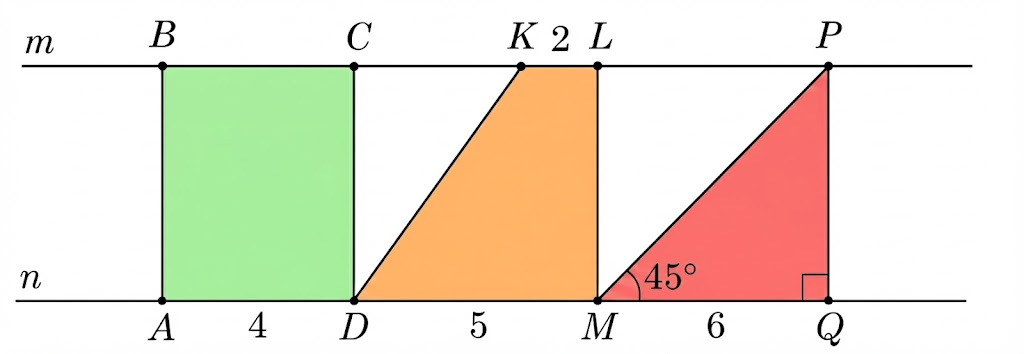
\includegraphics[scale=0.4]{parallel_lines_rect_trap_triangle.png}
\end{flushright}
\end{center}

\nmtnobreak
\nopagebreak\nbvspace{0.3cm}
\begin{minipage}[t]{0.55\textwidth}
\noindent
\begin{minipage}[t]{0.46\linewidth}
\matchHead{Фігура}
\matchItem{1}{Прямокутник $ABCD$}
\matchItem{2}{Трапеція $DKLM$}
\matchItem{3}{Трикутник $MQP$}
\end{minipage}%
\hfill
\begin{minipage}[t]{0.5\linewidth}
\matchHead{Площа фігури}
\matchItem{А}{12}
\matchItem{Б}{18}
\matchItem{В}{21}
\matchItem{Г}{24}
\matchItem{Д}{36}
\end{minipage}

\nopagebreak\nbvspace{0.3cm}
\hfill\matchingGrid
\end{minipage}
\hfill
\par\penalty-20\vspace{0.25cm}
\end{samepage}

\begin{samepage}
\needspace{0.45\textheight}\typeTitle{Площі фігур на папері в клітинку}
% НМТ 2026, сесія 18.06, завдання №18 --- основна тема: Трикутники
\zadtask{На папері у клітинку зображено точки $A$, $B$, $C$, $K$, $L$ та $M$ (див. рисунок). Кожна клітинка~--- квадрат площею $1$~см$^2$. Установіть відповідність між фігурою \mbox{(1--3)} та її площею \mbox{(А--Д)}. \nmtyear{2026}\par
\nopagebreak\nbvspace{0.3cm}
\begin{center}
\begin{nmtfit}\begin{tikzpicture}[scale=0.55, thick, line join=round]
    \draw[step=1cm, gray!40, thin] (-1.5,-1.5) grid (10.5,5.5);
    % як в оригіналі (с. 110): висота 4 клітинки, C над M; зеленим -- AK, BL, CM, AC, KM
    \coordinate (A) at (1,4);
    \coordinate (B) at (3,4);
    \coordinate (C) at (6,4);
    \coordinate (K) at (0,0);
    \coordinate (L) at (2,0);
    \coordinate (M) at (6,0);
    \draw[thick, green!55!black] (K) -- (A) -- (C) -- (M) -- cycle;
    \draw[thick, green!55!black] (L) -- (B);
    \foreach \p/\lab/\pos in {A/A/above left, B/B/above, C/C/above, K/K/below left, L/L/below, M/M/below} {
        \fill (\p) circle (2.5pt);
        \node[\pos, font=\scriptsize] at (\p) {$\lab$};
    }
    \draw[thick] (8,3) rectangle (9,4);
    \node[right, font=\scriptsize] at (9,3.5) {$1$~см$^2$};
\end{tikzpicture}\end{nmtfit}
\end{center}
\nopagebreak\nbvspace{0.2cm}
\noindent
\matchingLayout{
\matchHead{Фігура}
\matchItem{1}{$ACM$}
\matchItem{2}{$ABLK$}
\matchItem{3}{$BCML$}
}{
\matchHead{Площа фігури}
\matchItem{А}{$8$~см$^2$}
\matchItem{Б}{$10$~см$^2$}
\matchItem{В}{$12$~см$^2$}
\matchItem{Г}{$14$~см$^2$}
\matchItem{Д}{$16$~см$^2$}
}{
\matchingGrid
}
}
% Відповідь: 1--Б,\ \ 2--А,\ \ 3--Г
\par\penalty-20
\end{samepage}

\begin{samepage}
\needspace{0.45\textheight}\typeTitle{Авторські аналоги за зразком НМТ}
\zadtask{На рисунку зображено ромб $ABCD$, рівносторонній трикутник $CDK$ і прямокутний трикутник $AKN$ ($\angle AKN = 90^\circ$), що лежать в одній площині. Точки $A$, $D$ і $K$ лежать на одній прямій, катет $KN$ дорівнює меншій діагоналі ромба. Установіть відповідність між геометричною фігурою \mbox{(1--3)} та її площею \mbox{(А--Д)}, якщо $AK = 12$~см.
\par\nopagebreak\nbvspace{0.3cm}
\begin{center}
\begin{nmtfit}\begin{tikzpicture}[scale=0.4, thick, line join=round]
    \coordinate (A) at (0,0);
    \coordinate (D) at (6,0);
    \coordinate (K) at (12,0);
    \coordinate (B) at (3,5.196);
    \coordinate (C) at (9,5.196);
    \coordinate (N) at (12,-6);
    \filldraw[fill=yearOrange!20, draw=black] (A) -- (B) -- (C) -- (D) -- cycle;
    \filldraw[fill=mainGreen!20, draw=black] (D) -- (C) -- (K) -- cycle;
    \filldraw[fill=gray!20, draw=black] (A) -- (K) -- (N) -- cycle;
    \draw[dashed, thin] (B) -- (D);
    \draw[thin] (11.3,0) -- (11.3,-0.7) -- (12,-0.7);
    \node[left] at (A) {$A$};
    \node[above left] at (B) {$B$};
    \node[above right] at (C) {$C$};
    \node[below] at (D) {$D$};
    \node[right] at (K) {$K$};
    \node[below] at (N) {$N$};
\end{tikzpicture}\end{nmtfit}
\end{center}
\nopagebreak\nbvspace{0.2cm}
\noindent
\matchingLayout{
\matchHead{Геометрична фігура}
\matchItem{1}{трикутник $CDK$}
\matchItem{2}{трикутник $AKN$}
\matchItem{3}{ромб $ABCD$}
}{
\matchHead{Площа фігури}
\matchItem{А}{$36$~см$^2$}
\matchItem{Б}{$72$~см$^2$}
\matchItem{В}{$9\sqrt{3}$~см$^2$}
\matchItem{Г}{$18\sqrt{3}$~см$^2$}
\matchItem{Д}{$36\sqrt{3}$~см$^2$}
}{
\matchingGrid
}}
\end{samepage}

\begin{samepage}
\noindent
\begin{minipage}[c]{0.55\textwidth}
\zadnum У прямокутнику $ABCD$ $AB=6$~см, $AD=10$~см, $O$ -- точка перетину діагоналей, точка $K$ лежить на стороні $AD$, $AK=4$~см (див. рисунок). Установіть відповідність між трикутником \mbox{(1--3)} та його площею \mbox{(А--Д)}.
\end{minipage}\hfill
\begin{minipage}[c]{0.41\textwidth}\centering
\begin{nmtfit}\begin{tikzpicture}[scale=0.42, line join=round, line cap=round]
\coordinate (A) at (0.000,0.000);
\coordinate (B) at (0.000,6.000);
\coordinate (C) at (10.000,6.000);
\coordinate (D) at (10.000,0.000);
\coordinate (K) at (4.000,0.000);
\coordinate (O) at (5.000,3.000);
\draw[thick] (A) -- (B) -- (C) -- (D) -- cycle;
\draw[thick] (A) -- (C);
\draw[thick] (B) -- (D);
\draw[thick] (B) -- (K);
\node[circle, fill, inner sep=1.3pt] at (O) {};
\node[circle, fill, inner sep=1.3pt] at (K) {};
\node[font=\small, inner sep=0pt] at (-0.548,-0.548) {$A$};
\node[font=\small, inner sep=0pt] at (-0.548,6.548) {$B$};
\node[font=\small, inner sep=0pt] at (10.548,6.548) {$C$};
\node[font=\small, inner sep=0pt] at (10.548,-0.548) {$D$};
\node[font=\small, inner sep=0pt] at (3.809,-0.711) {$K$};
\node[font=\small, inner sep=0pt] at (5.000,2.238) {$O$};
\end{tikzpicture}\end{nmtfit}
\end{minipage}\par
\nmtnobreak
\nopagebreak\nbvspace{0.3cm}
\noindent
\matchingLayout{
\matchHead{Трикутник}
\matchItem{1}{$ABD$}
\matchItem{2}{$ABK$}
\matchItem{3}{$BOC$}
}{
\matchHead{Площа трикутника}
\matchItem{А}{$12$~см$^2$}
\matchItem{Б}{$15$~см$^2$}
\matchItem{В}{$24$~см$^2$}
\matchItem{Г}{$30$~см$^2$}
\matchItem{Д}{$60$~см$^2$}
}{
\matchingGrid
}
\end{samepage}

\begin{samepage}
\noindent
\begin{minipage}[c]{0.55\textwidth}
\zadnum У паралелограмі $ABCD$ з вершини $B$ проведено висоту $BK$ до сторони $AD$ (див. рисунок), $AK=6$~см, $BK=8$~см, $KD=10$~см. Установіть відповідність між фігурою \mbox{(1--3)} та її площею \mbox{(А--Д)}.
\end{minipage}\hfill
\begin{minipage}[c]{0.41\textwidth}\centering
\begin{nmtfit}\begin{tikzpicture}[scale=0.22, line join=round, line cap=round]
\coordinate (A) at (0.000,0.000);
\coordinate (B) at (6.000,8.000);
\coordinate (C) at (22.000,8.000);
\coordinate (D) at (16.000,0.000);
\coordinate (K) at (6.000,0.000);
\draw[thick] (A) -- (B) -- (C) -- (D) -- cycle;
\draw[thick] (B) -- (K);
\pic[draw, angle radius=0.2cm] {right angle = D--K--B};
\node[font=\small, inner sep=0pt] at (-1.047,-1.047) {$A$};
\node[font=\small, inner sep=0pt] at (6.000,9.273) {$B$};
\node[font=\small, inner sep=0pt] at (23.047,9.047) {$C$};
\node[font=\small, inner sep=0pt] at (17.047,-1.047) {$D$};
\node[font=\small, inner sep=0pt] at (6.000,-1.273) {$K$};
\end{tikzpicture}\end{nmtfit}
\end{minipage}\par
\nmtnobreak
\nopagebreak\nbvspace{0.3cm}
\noindent
\matchingLayout{
\matchHead{Фігура}
\matchItem{1}{паралелограм $ABCD$}
\matchItem{2}{трикутник $ABK$}
\matchItem{3}{трапеція $KBCD$}
}{
\matchHead{Площа фігури}
\matchItem{А}{$24$~см$^2$}
\matchItem{Б}{$48$~см$^2$}
\matchItem{В}{$80$~см$^2$}
\matchItem{Г}{$104$~см$^2$}
\matchItem{Д}{$128$~см$^2$}
}{
\matchingGrid
}
\end{samepage}

\begin{samepage}
\zadtask{На папері в клітинку зображено трикутник $KLM$, паралелограм $ABCD$ і трапецію $PQRS$ (див. рисунок). Площа однієї клітинки дорівнює $1$~см$^2$. Установіть відповідність між фігурою \mbox{(1--3)} та її площею \mbox{(А--Д)}.}
\nmtnobreak
\nopagebreak\nbvspace{0.3cm}
\begin{center}\begin{nmtfit}\begin{tikzpicture}[scale=0.32, line join=round, line cap=round]
\draw[gray!45, very thin] (-0.5,-0.5) grid (24.5,4.5);
\coordinate (K) at (0.000,0.000);
\coordinate (L) at (6.000,0.000);
\coordinate (M) at (2.000,4.000);
\coordinate (A) at (8.000,0.000);
\coordinate (B) at (10.000,4.000);
\coordinate (C) at (16.000,4.000);
\coordinate (D) at (14.000,0.000);
\coordinate (P) at (18.000,0.000);
\coordinate (Q) at (20.000,4.000);
\coordinate (R) at (22.000,4.000);
\coordinate (S) at (24.000,0.000);
\draw[thick] (K) -- (L) -- (M) -- cycle;
\draw[thick] (A) -- (B) -- (C) -- (D) -- cycle;
\draw[thick] (P) -- (Q) -- (R) -- (S) -- cycle;
\node[font=\small, inner sep=0pt] at (-0.000,-0.875) {$K$};
\node[font=\small, inner sep=0pt] at (6.000,-0.875) {$L$};
\node[font=\small, inner sep=0pt] at (2.000,4.875) {$M$};
\node[font=\small, inner sep=0pt] at (8.000,-0.875) {$A$};
\node[font=\small, inner sep=0pt] at (10.000,4.875) {$B$};
\node[font=\small, inner sep=0pt] at (16.000,4.875) {$C$};
\node[font=\small, inner sep=0pt] at (14.000,-0.875) {$D$};
\node[font=\small, inner sep=0pt] at (18.000,-0.875) {$P$};
\node[font=\small, inner sep=0pt] at (20.000,4.875) {$Q$};
\node[font=\small, inner sep=0pt] at (22.000,4.875) {$R$};
\node[font=\small, inner sep=0pt] at (24.000,-0.875) {$S$};
\end{tikzpicture}\end{nmtfit}\end{center}
\nmtnobreak
\nopagebreak\nbvspace{0.3cm}
\noindent
\matchingLayout{
\matchHead{Фігура}
\matchItem{1}{трикутник $KLM$}
\matchItem{2}{паралелограм $ABCD$}
\matchItem{3}{трапеція $PQRS$}
}{
\matchHead{Площа фігури}
\matchItem{А}{$8$~см$^2$}
\matchItem{Б}{$12$~см$^2$}
\matchItem{В}{$16$~см$^2$}
\matchItem{Г}{$24$~см$^2$}
\matchItem{Д}{$32$~см$^2$}
}{
\matchingGrid
}
\end{samepage}

\clearpage
\sectionTitle{Відповіді}

\noindent{\small\color{gray!80!black}Для кожного завдання -- літери відповідей для пунктів 1, 2, 3. Відповіді обчислено й звірено з офіційними ключами там, де вони є.}\par\vspace{0.3cm}

\begin{multicols}{5}\noindent
\mbox{1~--- АБВ}\par
\mbox{2~--- ВАГ}\par
\mbox{3~--- ВГА}\par
\mbox{4~--- ГВД}\par
\mbox{5~--- АБВ}\par
\mbox{6~--- ГВБ}\par
\mbox{7~--- БАГ}\par
\mbox{8~--- ВАГ}\par
\mbox{9~--- ГАБ}\par
\mbox{10~--- ДАГ}\par
\mbox{11~--- БГВ}
\end{multicols}

\noindent{\small\color{gray!80!black}8--11~--- авторські аналоги.}\par

\end{document}
